\documentclass[conf]{new-aiaa}
%\documentclass[journal]{new-aiaa} for journal papers
\usepackage[utf8]{inputenc}

\usepackage{graphicx}
\usepackage{amsmath}
\usepackage[version=4]{mhchem}
\usepackage{siunitx}
\usepackage{longtable,tabularx,booktabs}
\graphicspath{{figures/}}
\setlength\LTleft{0pt}
\sisetup{group-separator={,}, group-minimum-digits=4}

% Prevent LaTeX from creating float-only pages with large whitespace
\renewcommand{\floatpagefraction}{.82}
\renewcommand{\textfraction}{.08}
\renewcommand{\topfraction}{.9}
\renewcommand{\bottomfraction}{.7}

\title{Feasibility of Ion-Thruster-Only Maneuvering for a 6U CubeSat in Very Low Earth Orbit}

\author{Jonathan Stahl\footnote{Student, Department of Mechanical and Aerospace Engineering, The Ohio State University.},
David Franklin~II\textsuperscript{*},
Sai Vidyud Senthil Nathan\textsuperscript{*},
Aiden Reckamp\textsuperscript{*},
Thanadis Charoenrujijin\textsuperscript{*},
and Connor Lashley\textsuperscript{*}}
\affil{The Ohio State University, Columbus, Ohio 43210}

\begin{document}

\maketitle

\begin{abstract}
This paper evaluates whether ion thrusters alone can support both agile attitude maneuvers and sustained operation for a \SI{12}{\kilogram}, 6U CubeSat in very low Earth orbit (VLEO). The study combines a minimax attitude-slew model, target-of-opportunity tracking simulations, and a free-molecular aerodynamic compensation survey. A representative actuator-force budget of \SI{145}{\milli\newton} is applied through moment arms of $[0.3,\,0.3,\,0.2]$~m. The instantaneous maneuver results are favorable: a \SI{180}{\degree} rest-to-rest slew completes in \SI{6.13}{\second} on the worst principal axis and \SI{3.97}{\second} on the optimal axis, while illustrative \SI{200}{\kilo\meter} tracking and slew-to-track cases require only \SI{0.685}{\milli\newton} and \SI{0.617}{\milli\newton} peak actuator force, respectively. An aerodynamic-aware match-time scan places the slew-to-track handoff at \SI{193}{\second} and reveals that the required actuator force is dominated by aerodynamic compensation rather than by the maneuver itself. However, sustained VLEO operation is endurance-limited rather than peak-force-limited. For a \SI{1.5}{\kilogram} usable propellant allocation, the nadir-pointing mission life at \SI{170}{\kilo\meter} is only 6.74~days at $I_{sp}=\SI{760}{\second}$ and 26.62~days at $I_{sp}=\SI{3000}{\second}$; even at \SI{200}{\kilo\meter}, the same cases yield only 18.70 and 73.82~days. An advanced $I_{sp}=\SI{19300}{\second}$ case extends life substantially but is not representative of current CubeSat-class ion propulsion. The results demonstrate that ion thrusters can satisfy the instantaneous force demand for VLEO maneuvers, but ion-thruster-only architectures are not well suited to sustained VLEO missions unless paired with higher propellant mass, substantially higher specific impulse, or hybrid control architectures.
\end{abstract}

%======================================================================================
\section{Nomenclature}

{\renewcommand\arraystretch{1.0}
\noindent\begin{longtable*}{@{}l @{\quad=\quad} l@{}}
$\boldsymbol{\beta}$ & quaternion attitude vector \\
$\boldsymbol{\omega}$ & angular velocity vector, rad/s \\
$\boldsymbol{\tau}$ & total external torque vector \\
$\tau_i$ & body-axis control torque component \\
$F_{\max}$ & actuator force budget per controlled axis \\
$\bar{F}_{\mathrm{tot}}$ & orbit-averaged total thruster force \\
$g_0$ & standard gravitational acceleration, \SI{9.80665}{\meter\per\second\squared} \\
$\mathbf{I}_{C}$ & spacecraft body-frame inertia matrix \\
$I_{sp}$ & specific impulse \\
$L_i$ & effective moment arm for body axis $i$ \\
$m_{\mathrm{prop}}$ & usable propellant mass \\
$\dot{m}$ & propellant mass flow rate \\
$T_{\min}$ & minimum rest-to-rest slew time \\
$t_{\mathrm{life}}$ & propellant-limited mission life \\
$\theta$ & angular separation between initial and target attitudes \\
$\gamma$ & minimax body-axis force demand, $\max_i |\tau_i|/L_i$ \\
TOO & target of opportunity \\
VLEO & very low Earth orbit
\end{longtable*}}

%======================================================================================
\section{Introduction} \label{sec:introduction}

Very low Earth orbit (VLEO) offers compelling advantages for Earth observation missions, including reduced launch costs for heavier payloads, enhanced geospatial imaging resolution, and improved signal-to-noise ratios for ground-directed sensors. These characteristics make VLEO particularly attractive for rapid-response applications such as wildfire detection, natural disaster coordination, and atmospheric and space-weather monitoring. However, operating below approximately \SI{300}{\kilo\meter} introduces severe environmental challenges: residual atmospheric density generates substantial aerodynamic drag that continuously depletes orbital energy, while the atomic-oxygen flux accelerates material degradation of exposed spacecraft surfaces.

JAXA's TSUBAME (SLATS) technology demonstrator underscores both the promise and the difficulty of the regime. TSUBAME reached a record low sustained orbital altitude of \SI{167.4}{\kilo\meter}, and JAXA reported that the \SIrange{200}{300}{\kilo\meter} environment can impose atmospheric and atomic-oxygen exposure roughly three orders of magnitude more severe than that encountered in conventional Earth-observation orbits \cite{jaxavariety,jaxaterminate}. Sustaining both orbit and attitude in this environment requires continuous propulsive authority, making ion thrusters a natural candidate owing to their high specific impulse and long operational life.

Representative ion-thruster hardware already spans a wide performance range. In terms of thrust, NASA's NEXT-C operates over approximately \SIrange{25}{235}{\milli\newton} \cite{nextc}, while QinetiQ's T6 has published operating points up to approximately \SI{145}{\milli\newton} \cite{t6eval}. In terms of specific impulse, electrospray devices can operate near $I_{sp}=\SI{760}{\second}$ \cite{krejci2017}, conventional low-power ion engines have historically occupied the \SIrange{2000}{3000}{\second} range \cite{nasalowpower}, and ESA's DS4G concept demonstrates a substantially higher upper bound near \SI{19300}{\second} \cite{ds4goverview}. However, ion thrusters produce low thrust relative to chemical systems, and their substantial electrical power requirements complicate accommodation on compact platforms \cite{ionpropulsion,ionmotors}.

The central engineering question is not whether ion thrusters can generate thrust, but whether they alone can provide sufficient instantaneous control authority for agile VLEO maneuvers while simultaneously preserving useful mission life. Peak force determines whether a given maneuver is feasible at all, whereas cumulative propellant consumption determines whether the mission can remain in the useful VLEO altitude band long enough to fulfill its objectives.

This paper evaluates that trade for a \SI{12}{\kilogram} 6U CubeSat through four linked studies:
\begin{enumerate}
    \item a force-limited analytic and numerical rest-to-rest slew sweep,
    \item an altitude sweep for nadir-pass target-of-opportunity (TOO) tracking with aerodynamic compensation,
    \item deterministic \SI{200}{\kilo\meter} TOO tracking and slew-to-track demonstrations, and
    \item a propellant-limited endurance sweep for continuous aerodynamic compensation under nadir-pointing operation.
\end{enumerate}

The central finding is that ion thrusters can satisfy the instantaneous force demand for the modeled VLEO maneuvers, but an ion-thruster-only architecture becomes life-limited at practically interesting VLEO altitudes, suggesting that hybrid control strategies or substantially higher-performance propulsion are necessary for operationally viable missions.

%======================================================================================
\section{Background} \label{sec:background}

%--------------------------------------------------------------------------------------
\subsection{Ion propulsion in the context of VLEO attitude control} \label{subsec:ion_propulsion}

Ion thrusters have traditionally served deep-space propulsion and long-duration station-keeping, where their high specific impulse translates directly into reduced propellant mass \cite{ionpropulsion}. Repurposing them for VLEO attitude control introduces a distinct challenge: rapid reorientation toward ground targets demands agile torque authority that low-thrust actuators may struggle to provide. The stringent mass and volume constraints of small VLEO satellites, combined with the substantial electrical power that ion systems require, further complicate accommodation on compact platforms \cite{ionmotors}. This study therefore quantifies whether the modest thrust levels characteristic of ion propulsion can provide adequate torque $\boldsymbol{\tau}$ for the slew and tracking maneuvers described in Section~\ref{sec:methodology}.

%--------------------------------------------------------------------------------------
\subsection{Attitude kinematics} \label{subsec:attitude_kinematics}

This study adopts a quaternion parameterization for spacecraft attitude. Among the common representations (Euler angles, direction cosine matrices, and quaternions \cite{kumar_attitudeparam}), quaternions offer a singularity-free, minimal-redundancy description using only four parameters, which is well suited to the large-angle slew maneuvers considered here.

A quaternion $\boldsymbol{\beta} = [q_0,\, q_1,\, q_2,\, q_3]^T$ encodes the orientation of the body frame relative to a reference frame using the scalar-first convention. The kinematic differential equation relating the quaternion rate to the body angular velocity $\boldsymbol{\omega}$ is
\begin{equation} \label{eq:qdot}
    \dot{\boldsymbol{\beta}} = \frac{1}{2}\,B[\boldsymbol{\beta}]
    \begin{pmatrix} 0 \\ \boldsymbol{\omega} \end{pmatrix},
\end{equation}
where $B[\boldsymbol{\beta}]$ is a $4\times4$ matrix constructed from the quaternion elements. Because numerical integration introduces norm drift, the quaternion is renormalized after each propagation step to enforce the unit-norm constraint $\|\boldsymbol{\beta}\| = 1$.

%--------------------------------------------------------------------------------------
\subsection{Attitude kinetics} \label{subsec:attitude_kinetics}

The rotational dynamics follow from the angular momentum principle \cite{kumar_eulerianmechanics}. For a rigid body with inertia matrix $\mathbf{I}_C$ expressed in the body frame, the angular momentum about the center of mass is
\begin{equation} \label{eq:HC}
    \boldsymbol{H}_C = \mathbf{I}_C \,\boldsymbol{\omega}.
\end{equation}
Applying the transport theorem to express the inertial time derivative in the rotating body frame gives
\begin{equation} \label{eq:transport}
    \left(\frac{d\boldsymbol{H}_C}{dt}\right)_{\!\text{inertial}}
    = \left(\frac{d\boldsymbol{H}_C}{dt}\right)_{\!\text{body}}
    + \boldsymbol{\omega} \times \boldsymbol{H}_C.
\end{equation}
Setting the inertial rate of change equal to the total external torque $\boldsymbol{\tau}$ and substituting Eq.~\eqref{eq:HC} yields Euler's rotational equation:
\begin{equation} \label{eq:euler}
    \boldsymbol{\tau} = \mathbf{I}_C \,\dot{\boldsymbol{\omega}}
    + \boldsymbol{\omega} \times \bigl(\mathbf{I}_C \,\boldsymbol{\omega}\bigr).
\end{equation}
Rearranging for the angular acceleration gives the state-space form used throughout the simulations:
\begin{equation} \label{eq:wdot}
    \dot{\boldsymbol{\omega}} = \mathbf{I}_C^{-1}
    \Bigl(\boldsymbol{\tau}
    - \boldsymbol{\omega} \times \bigl(\mathbf{I}_C\,\boldsymbol{\omega}\bigr)\Bigr).
\end{equation}
Together, Eqs.~\eqref{eq:qdot} and~\eqref{eq:wdot} form the seven-state propagation system $[\boldsymbol{\beta};\,\boldsymbol{\omega}]$ used in all subsequent analyses.

%--------------------------------------------------------------------------------------
\subsection{Aerodynamic environment in VLEO} \label{subsec:aero_environment}

In VLEO, aerodynamic drag is the dominant environmental disturbance. Although the atmosphere is highly rarefied below \SI{300}{\kilo\meter}, residual gas density combined with orbital velocities exceeding \SI{7.5}{\kilo\meter\per\second} generates substantial drag forces and torques that continuously deplete orbital energy and perturb spacecraft attitude. These loads depend on atmospheric density, spacecraft velocity, exposed cross-sectional area, and the gas--surface interaction model. Because VLEO atmospheric density varies significantly with solar activity, geomagnetic conditions, and diurnal effects, the simulations in this study use dynamic atmospheric modeling rather than static density assumptions.

At the altitudes considered here, the mean free path of atmospheric molecules greatly exceeds the characteristic spacecraft dimension, placing the flow in the free-molecular regime (Knudsen number $\gg 1$). Under these conditions, gas--surface interaction models such as the Sentman or Cook formulations replace the inapplicable Navier--Stokes continuum framework, computing aerodynamic force and torque on each exposed panel individually.

Other environmental disturbances, including gravity-gradient torques, residual magnetic dipole interactions, and solar radiation pressure, are typically at least an order of magnitude smaller than aerodynamic torques at VLEO altitudes and are not modeled in this analysis.

%======================================================================================
\section{Methodology} \label{sec:methodology}

Figure~\ref{fig:workflow} provides an overview of the analysis workflow used in this study.

\begin{figure*}[!htb]
\centering
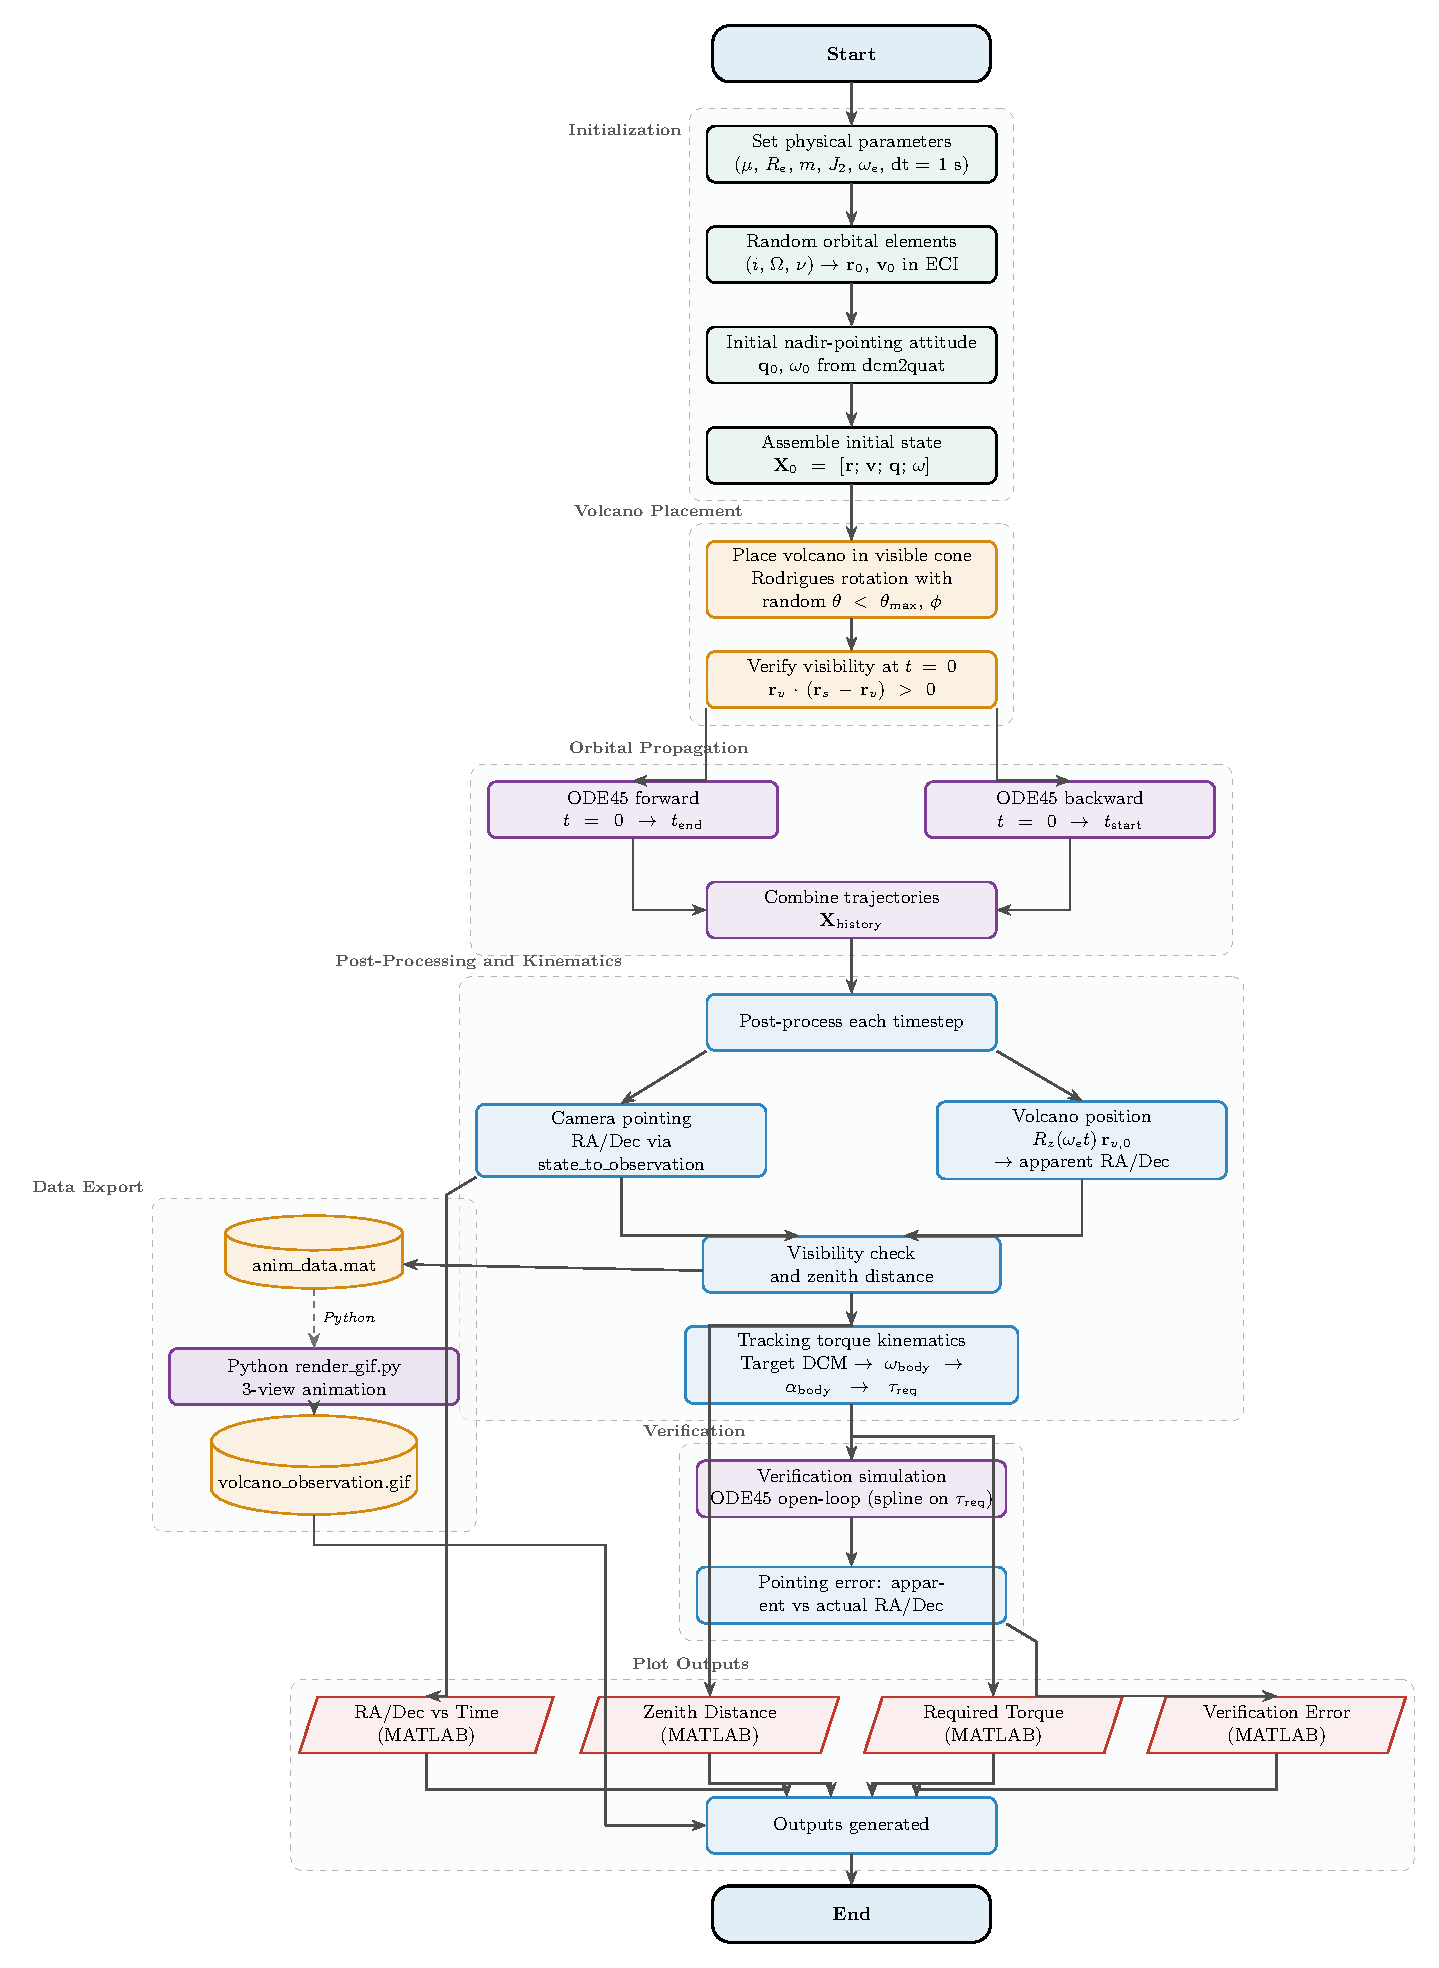
\includegraphics[width=0.75\textwidth]{workflow}
\caption{Overview of the analysis workflow. (Placeholder; to be replaced with final flowchart.)}
\label{fig:workflow}
\end{figure*}

%--------------------------------------------------------------------------------------
\subsection{Spacecraft and actuator model} \label{subsec:sc_model}

The reference vehicle is a $10 \times 20 \times 30$~cm, \SI{12}{\kilogram} 6U CubeSat. The principal inertia matrix is
\begin{equation}
    \mathbf{I}_{C} = \mathrm{diag}(0.13,\,0.10,\,0.05)~\si{\kilogram\meter\squared}.
\end{equation}
The actuation geometry is represented by effective moment arms $\mathbf{L} = [0.3,\,0.3,\,0.2]^T$~m, so that the body-axis force demand for a given torque vector is
\begin{equation}
    \gamma = \max_i \frac{|\tau_i|}{L_i}.
    \label{eq:gamma}
\end{equation}
Throughout this paper, the baseline actuator-force budget is $F_{\max}=\SI{145}{\milli\newton}$, chosen to be consistent with a high-end demonstrated ion-engine operating point \cite{t6eval}.

For rest-to-rest principal-axis maneuvers, the analytic minimum slew time is
\begin{equation}
    T_{\min,k} = 2\sqrt{\frac{\theta\, I_k}{L_k\, F_{\max}}},
    \label{eq:tmin}
\end{equation}
where $\theta$ is the rotation angle about principal axis~$k$. For finite-time slew-to-track transitions, a minimax boundary-value solver computes the torque history $\boldsymbol{\tau}(t)$ that minimizes the peak body-axis force demand, with each component $\tau_i$ converted to equivalent actuator force through Eq.~\eqref{eq:gamma}.

%--------------------------------------------------------------------------------------
\subsection{Scenario set} \label{subsec:scenarios}

Four scenario families are evaluated.

\textit{Rest-to-rest sweep.}\ \ The minimum slew duration is computed for angular separations from \SI{0.5}{\degree} to \SI{180}{\degree}, isolating the pure attitude-agility limit imposed by the force budget.

\textit{TOO altitude sweep.}\ \ A nadir-pass target-of-opportunity scenario places the ground target directly below the spacecraft at closest approach and computes the maximum actuator force required to maintain tracking throughout the visible pass. The sweep spans \SIrange{100}{200}{\kilo\meter} altitude.

\textit{Deterministic \SI{200}{\kilo\meter} demonstrations.}\ \ Two illustrative cases at \SI{200}{\kilo\meter} are simulated using a fixed scenario seed for reproducibility. The first case performs continuous TOO tracking; the second starts from a nadir-pointing hold, executes a finite-time minimax slew, and hands off into the tracking attitude and body rate. The seeded geometry is comparatively benign and should be interpreted as illustrative rather than worst-case.

\textit{Nadir-pointing endurance sweep.}\ \ Propellant-limited mission life is evaluated from \SIrange{150}{250}{\kilo\meter}. Each altitude point is averaged over three circular orbits with 120 samples per orbit. The survey assumes \SI{1.5}{\kilogram} usable propellant and evaluates three representative specific-impulse values: $I_{sp}=\SI{760}{\second}$ (electrospray-class lower bound \cite{krejci2017}), $I_{sp}=\SI{3000}{\second}$ (conventional ion-thruster class \cite{nasalowpower}), and $I_{sp}=\SI{19300}{\second}$ (advanced DS4G-class upper bound \cite{ds4goverview}).

%--------------------------------------------------------------------------------------
\subsection{Slew maneuver design} \label{subsec:slewing}

% TODO: Describe the slew control approach.
% Suggested content:
%   - Open-loop bang-bang / minimax torque profile design
%   - Nonlinear controller (proportional gain, feedforward)
%   - Linear controller and reference-point formulation
%   - How the solver produces the rest-to-rest and boundary-value slew solutions

%--------------------------------------------------------------------------------------
\subsection{Target tracking control} \label{subsec:tracking}

% TODO: Describe the tracking control approach.
% Suggested content:
%   - Reference trajectory derivation (pointing vector, frame completeness)
%   - Active feedback control law (PD or quaternion-error feedback)
%   - Handling of aerodynamic disturbance torque during tracking
%   - Noise injection / robustness considerations

%--------------------------------------------------------------------------------------
\subsection{Aerodynamic compensation and endurance model} \label{subsec:aero_model}

Aerodynamic loads are evaluated in the free-molecular regime using the Cook gas--surface interaction model. The endurance survey allocates both the aerodynamic force and the aerodynamic torque to an eight-thruster corner layout, then uses the orbit-averaged total scalar thruster force $\bar{F}_{\mathrm{tot}}$ to estimate propellant consumption and mission life:
\begin{equation}
    \dot{m} = \frac{\bar{F}_{\mathrm{tot}}}{I_{sp}\, g_0},
    \qquad
    t_{\mathrm{life}} = \frac{m_{\mathrm{prop}}}{\dot{m}}.
    \label{eq:life}
\end{equation}
This formulation is intentionally conservative: it does not consider whether a hybrid attitude-control architecture could reduce propellant consumption, but instead evaluates whether ion thrusters alone can both maneuver and sustain the vehicle in VLEO.

%======================================================================================

\begin{table*}[!htb]
\caption{Representative quantitative results from the VLEO ion-thruster feasibility study.}
\label{tab:key-results}
\centering
\begin{tabular}{p{0.62\textwidth}p{0.28\textwidth}}
\toprule
Metric & Value \\
\midrule
Worst-axis \SI{180}{\degree} rest-to-rest slew time at \SI{145}{\milli\newton} & \SI{6.13}{\second} \\
Optimal-axis \SI{180}{\degree} rest-to-rest slew time at \SI{145}{\milli\newton} & \SI{3.97}{\second} \\
Nadir-pass TOO tracking altitude where peak force crosses \SI{145}{\milli\newton} & \SI{112.7}{\kilo\meter} \\
Illustrative \SI{200}{\kilo\meter} TOO tracking peak force / max angular error & \SI{0.685}{\milli\newton} / \SI{0.010}{\degree} \\
Illustrative \SI{200}{\kilo\meter} slew-to-track peak force / post-match max pointing error & \SI{0.617}{\milli\newton} / \SI{0.0183}{\degree} \\
Mission life at \SI{170}{\kilo\meter} for $I_{sp} = [760,\, 3000,\, 19300]$~s & $[6.74,\, 26.62,\, 171.24]$~days \\
Mission life at \SI{200}{\kilo\meter} for $I_{sp} = [760,\, 3000,\, 19300]$~s & $[18.70,\, 73.82,\, 474.89]$~days \\
\bottomrule
\end{tabular}
\end{table*}

%======================================================================================
\section{Results} \label{sec:results}

%--------------------------------------------------------------------------------------
\subsection{Force-limited maneuver envelope}

Figure~\ref{fig:slew-sweep} presents the attitude-agility result for the rest-to-rest sweep. With the \SI{145}{\milli\newton} force budget, the minimum-time response is fast across the full angular-separation range. Even the worst principal axis completes a \SI{180}{\degree} slew in \SI{6.13}{\second}, while the optimal-axis maneuver completes in \SI{3.97}{\second}. The analytic and numerical solutions are in close agreement throughout, and no region of the sweep indicates that instantaneous slew authority is a limiting factor for the modeled 6U vehicle.

\begin{figure*}[!htb]
\centering
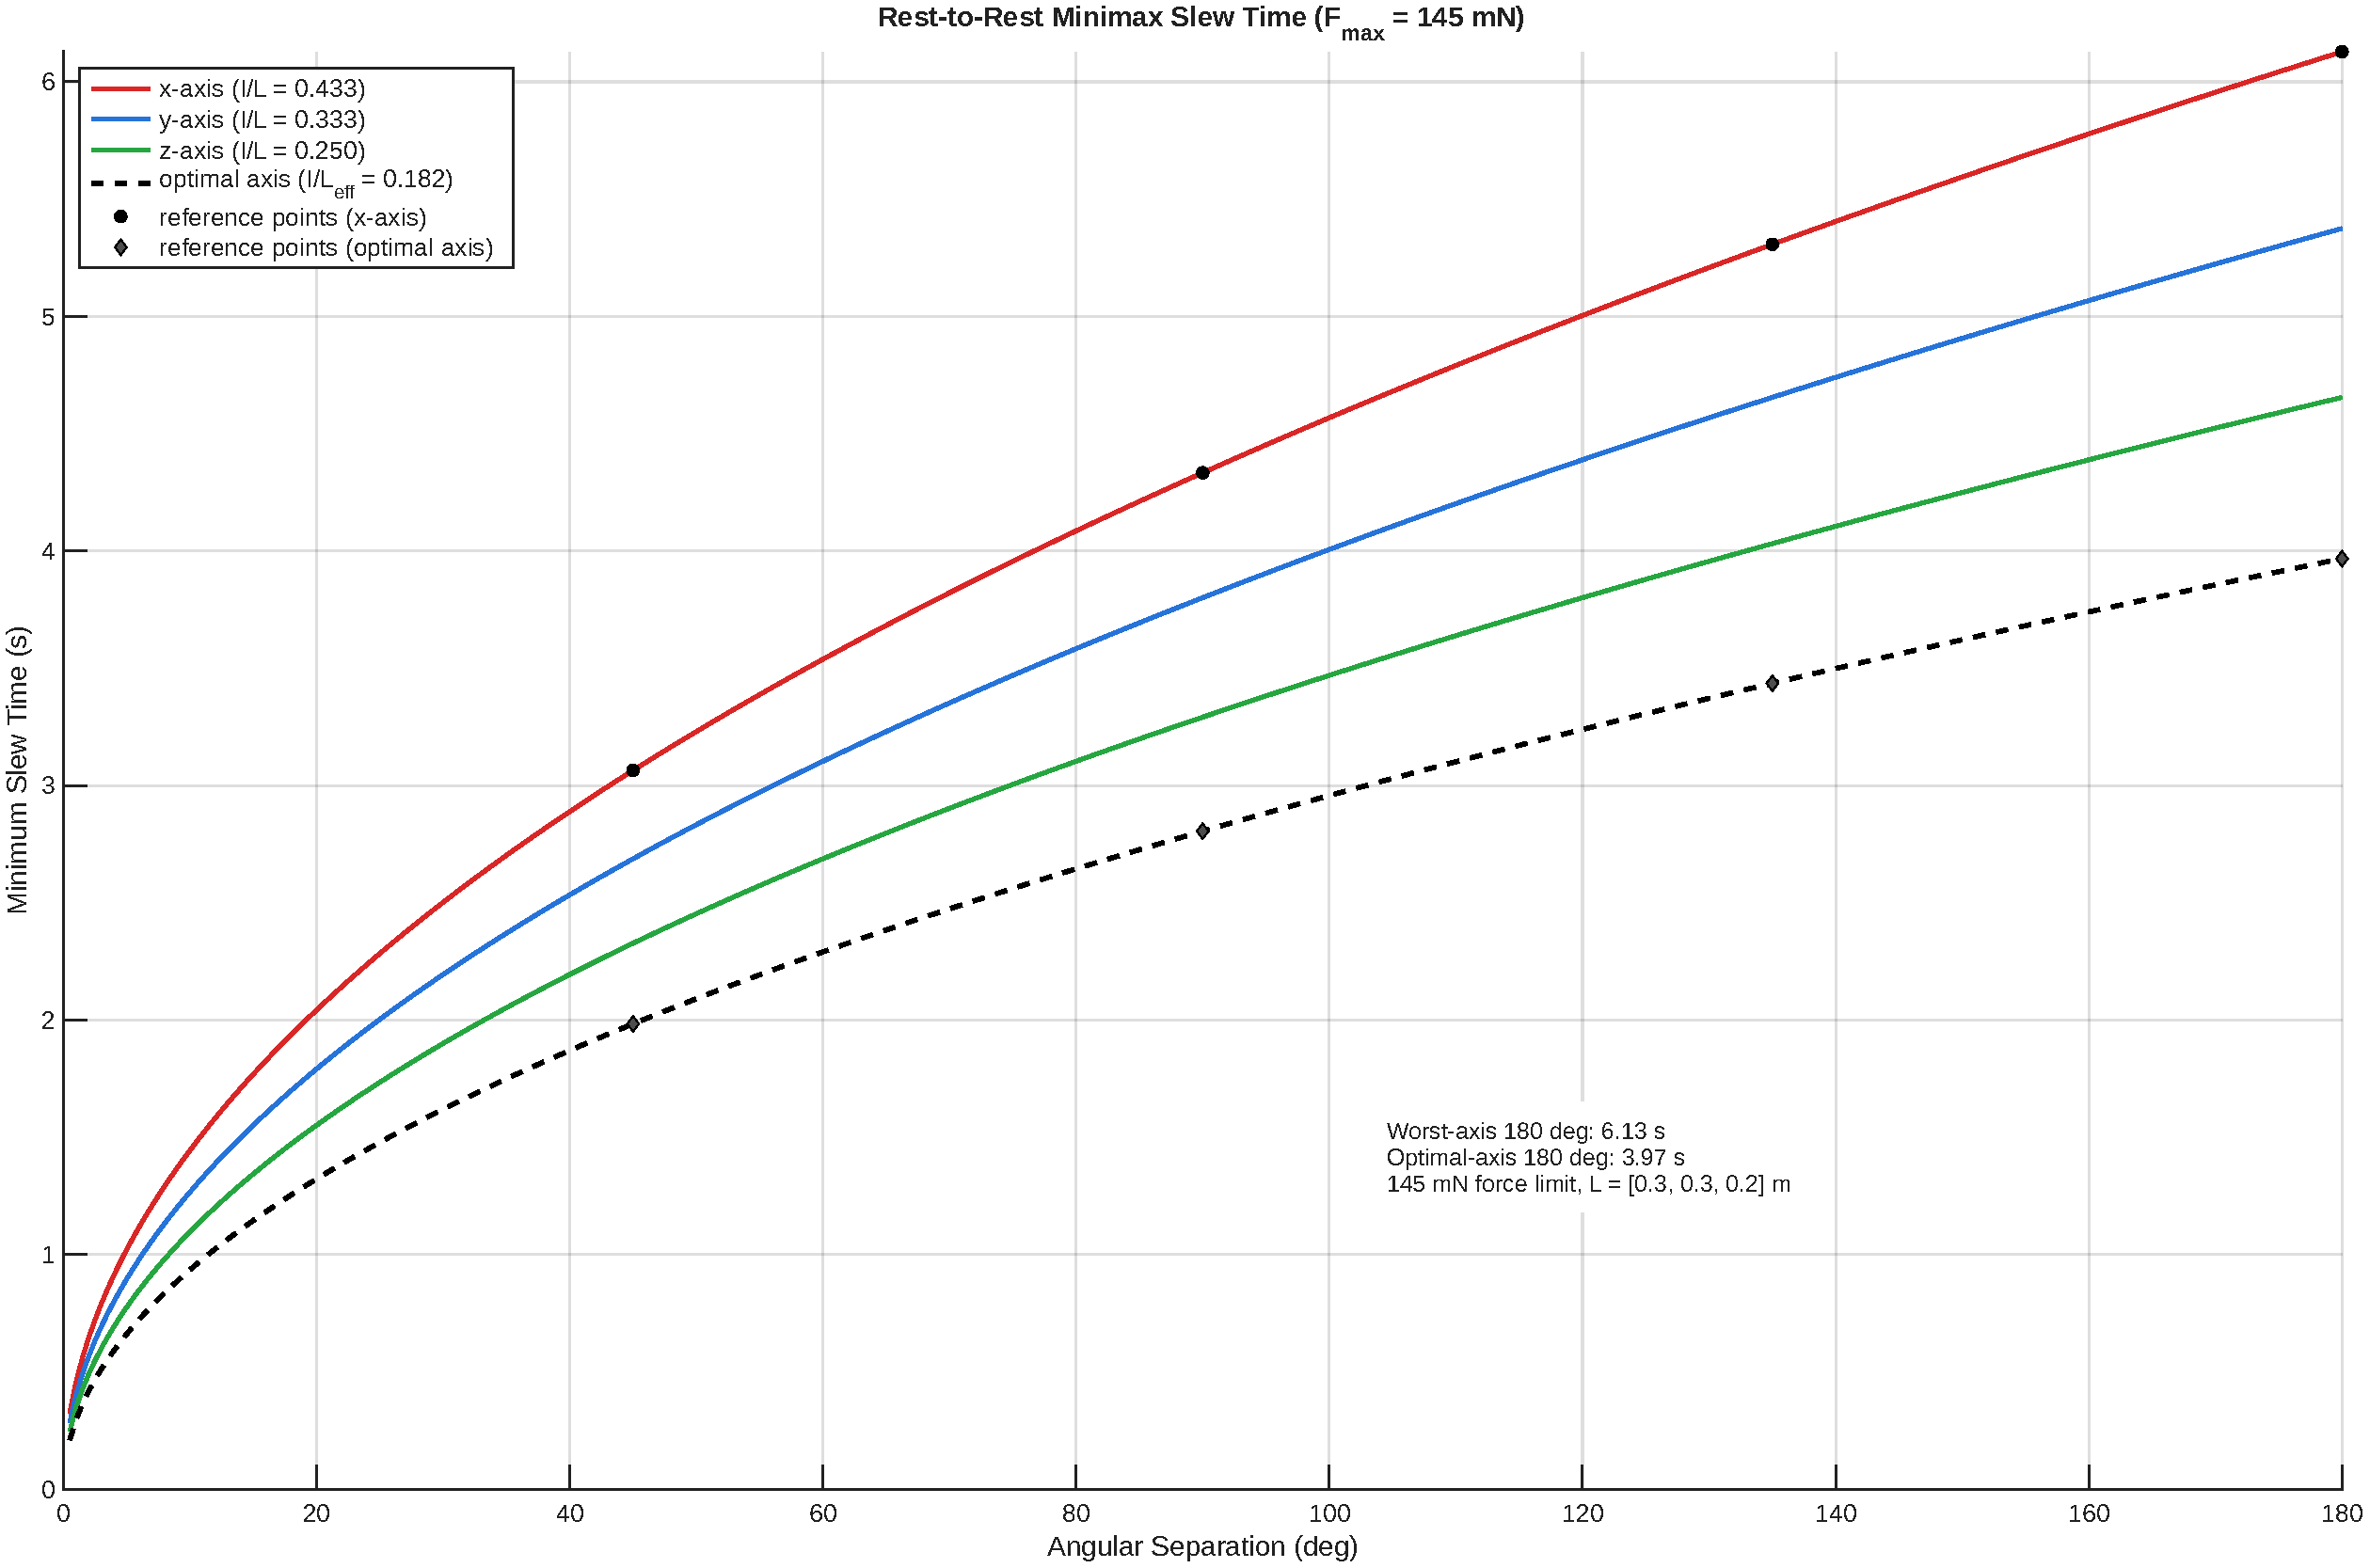
\includegraphics[width=0.75\textwidth]{force_limited_slew_sweep}
\caption{Force-limited minimum slew time versus angular separation for the \SI{12}{\kilogram} 6U reference vehicle. The \SI{145}{\milli\newton} force budget permits sub-\SI{7}{\second} rest-to-rest slews even for a worst-axis \SI{180}{\degree} maneuver.}
\label{fig:slew-sweep}
\end{figure*}

This result establishes that peak-force feasibility is not the binding constraint for the modeled vehicle. Were the system peak-force-limited, the subsequent VLEO analyses would be moot. Instead, the sweep confirms that a high-end ion-thruster-class force budget is already sufficient for rapid rigid-body reorientation across the full angular range.

%--------------------------------------------------------------------------------------
\subsection{Altitude-dependent TOO tracking feasibility}

Figure~\ref{fig:nadir-too-altitude} extends the force analysis to a more operationally representative scenario: nadir-pass TOO tracking with aerodynamic compensation. The peak force requirement is strongly altitude-dependent. The \SI{145}{\milli\newton} budget is exceeded at approximately \SI{112.7}{\kilo\meter}. Above that altitude, the required force decreases rapidly: \SI{55.2}{\milli\newton} at \SI{120}{\kilo\meter}, \SI{5.0}{\milli\newton} at \SI{150}{\kilo\meter}, and only \SI{0.94}{\milli\newton} at \SI{200}{\kilo\meter}.

\begin{figure*}[!htb]
\centering
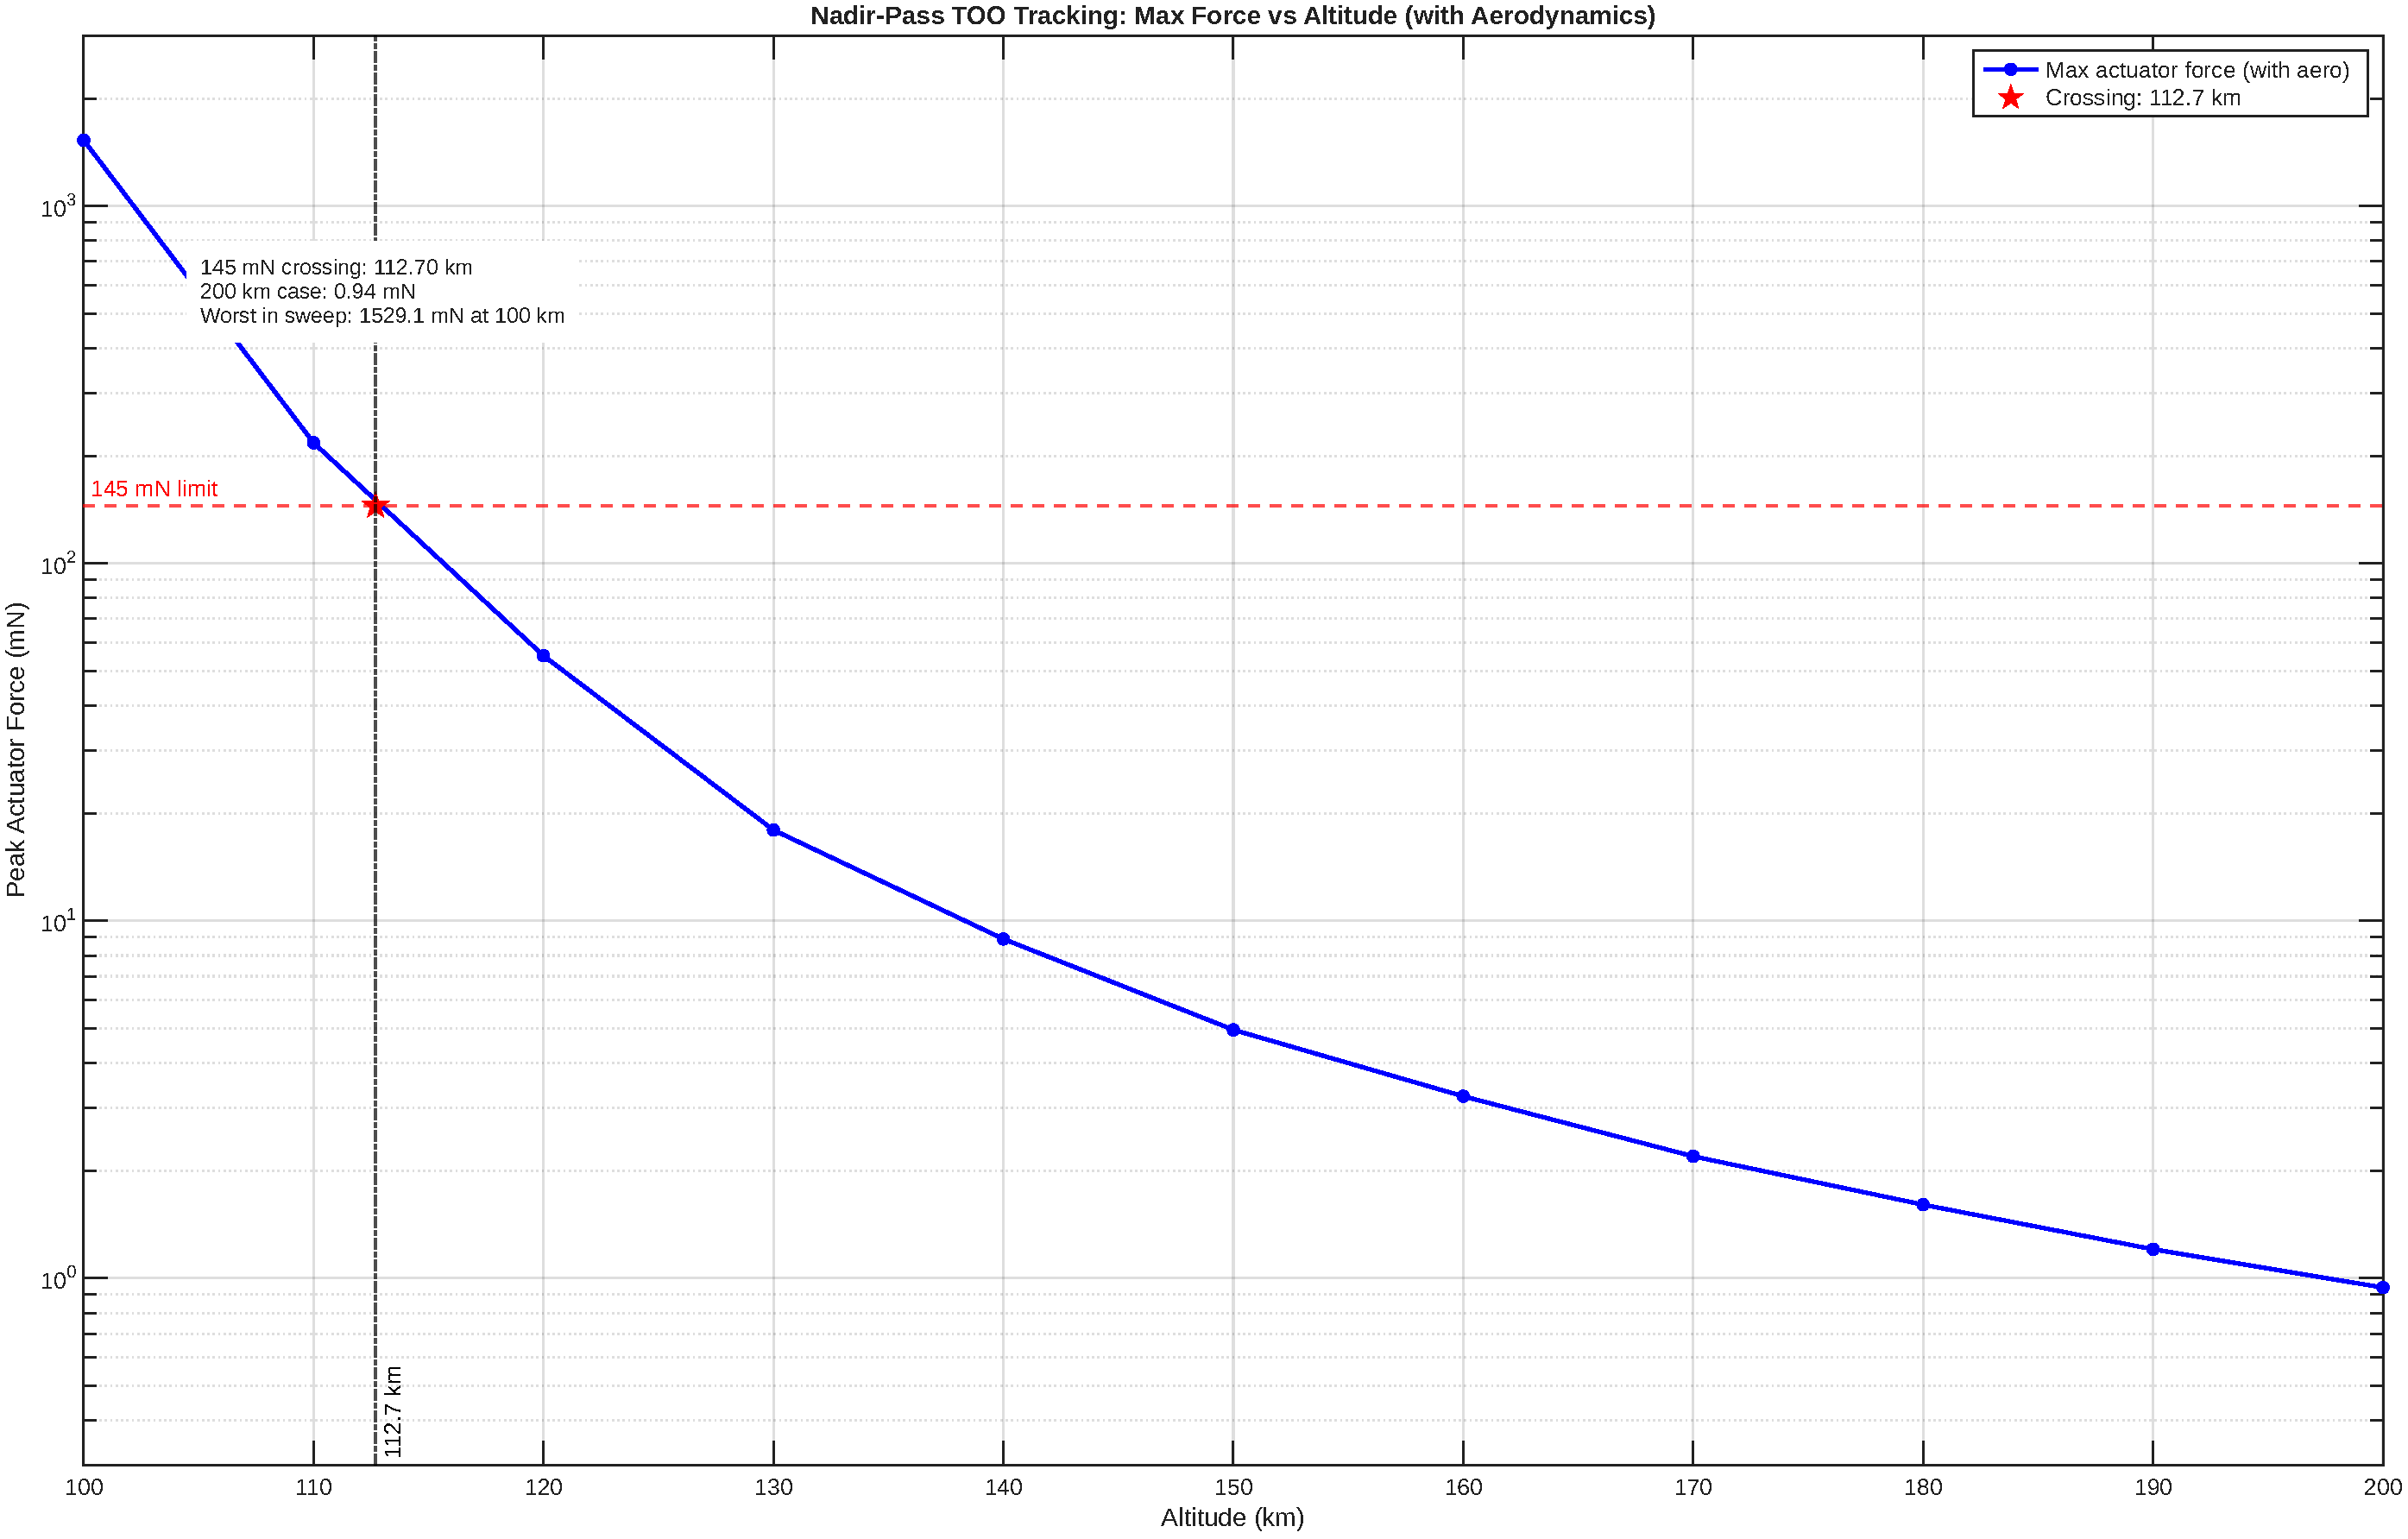
\includegraphics[width=0.75\textwidth]{nadir_too_force_vs_altitude}
\caption{Peak actuator force required for nadir-pass TOO tracking with aerodynamic compensation. The \SI{145}{\milli\newton} budget is exceeded only below approximately \SI{112.7}{\kilo\meter}.}
\label{fig:nadir-too-altitude}
\end{figure*}

This threshold establishes that above the deepest VLEO regime, the tracking problem is not peak-force-limited. An ion-thruster-class actuator can sustain the modeled nadir-pass tracking geometry without saturating, even after aerodynamic disturbances are included.

%--------------------------------------------------------------------------------------
\subsection{Illustrative \SI{200}{\kilo\meter} tracking and slew-to-track cases}

While the altitude sweep addresses the envelope question, deterministic time histories provide additional insight into the maneuver structure. Figure~\ref{fig:tracking-case} shows the seeded \SI{200}{\kilo\meter} continuous-tracking case. The peak actuator force is \SI{0.685}{\milli\newton}, corresponding to 0.47\% of the \SI{145}{\milli\newton} budget, and the open-loop verification error remains near \SI{0.010}{\degree}. Although this particular seed represents a comparatively favorable geometry, the result demonstrates that the force demand is far below the representative ion-thruster limit.

\begin{figure*}[!htb]
\centering
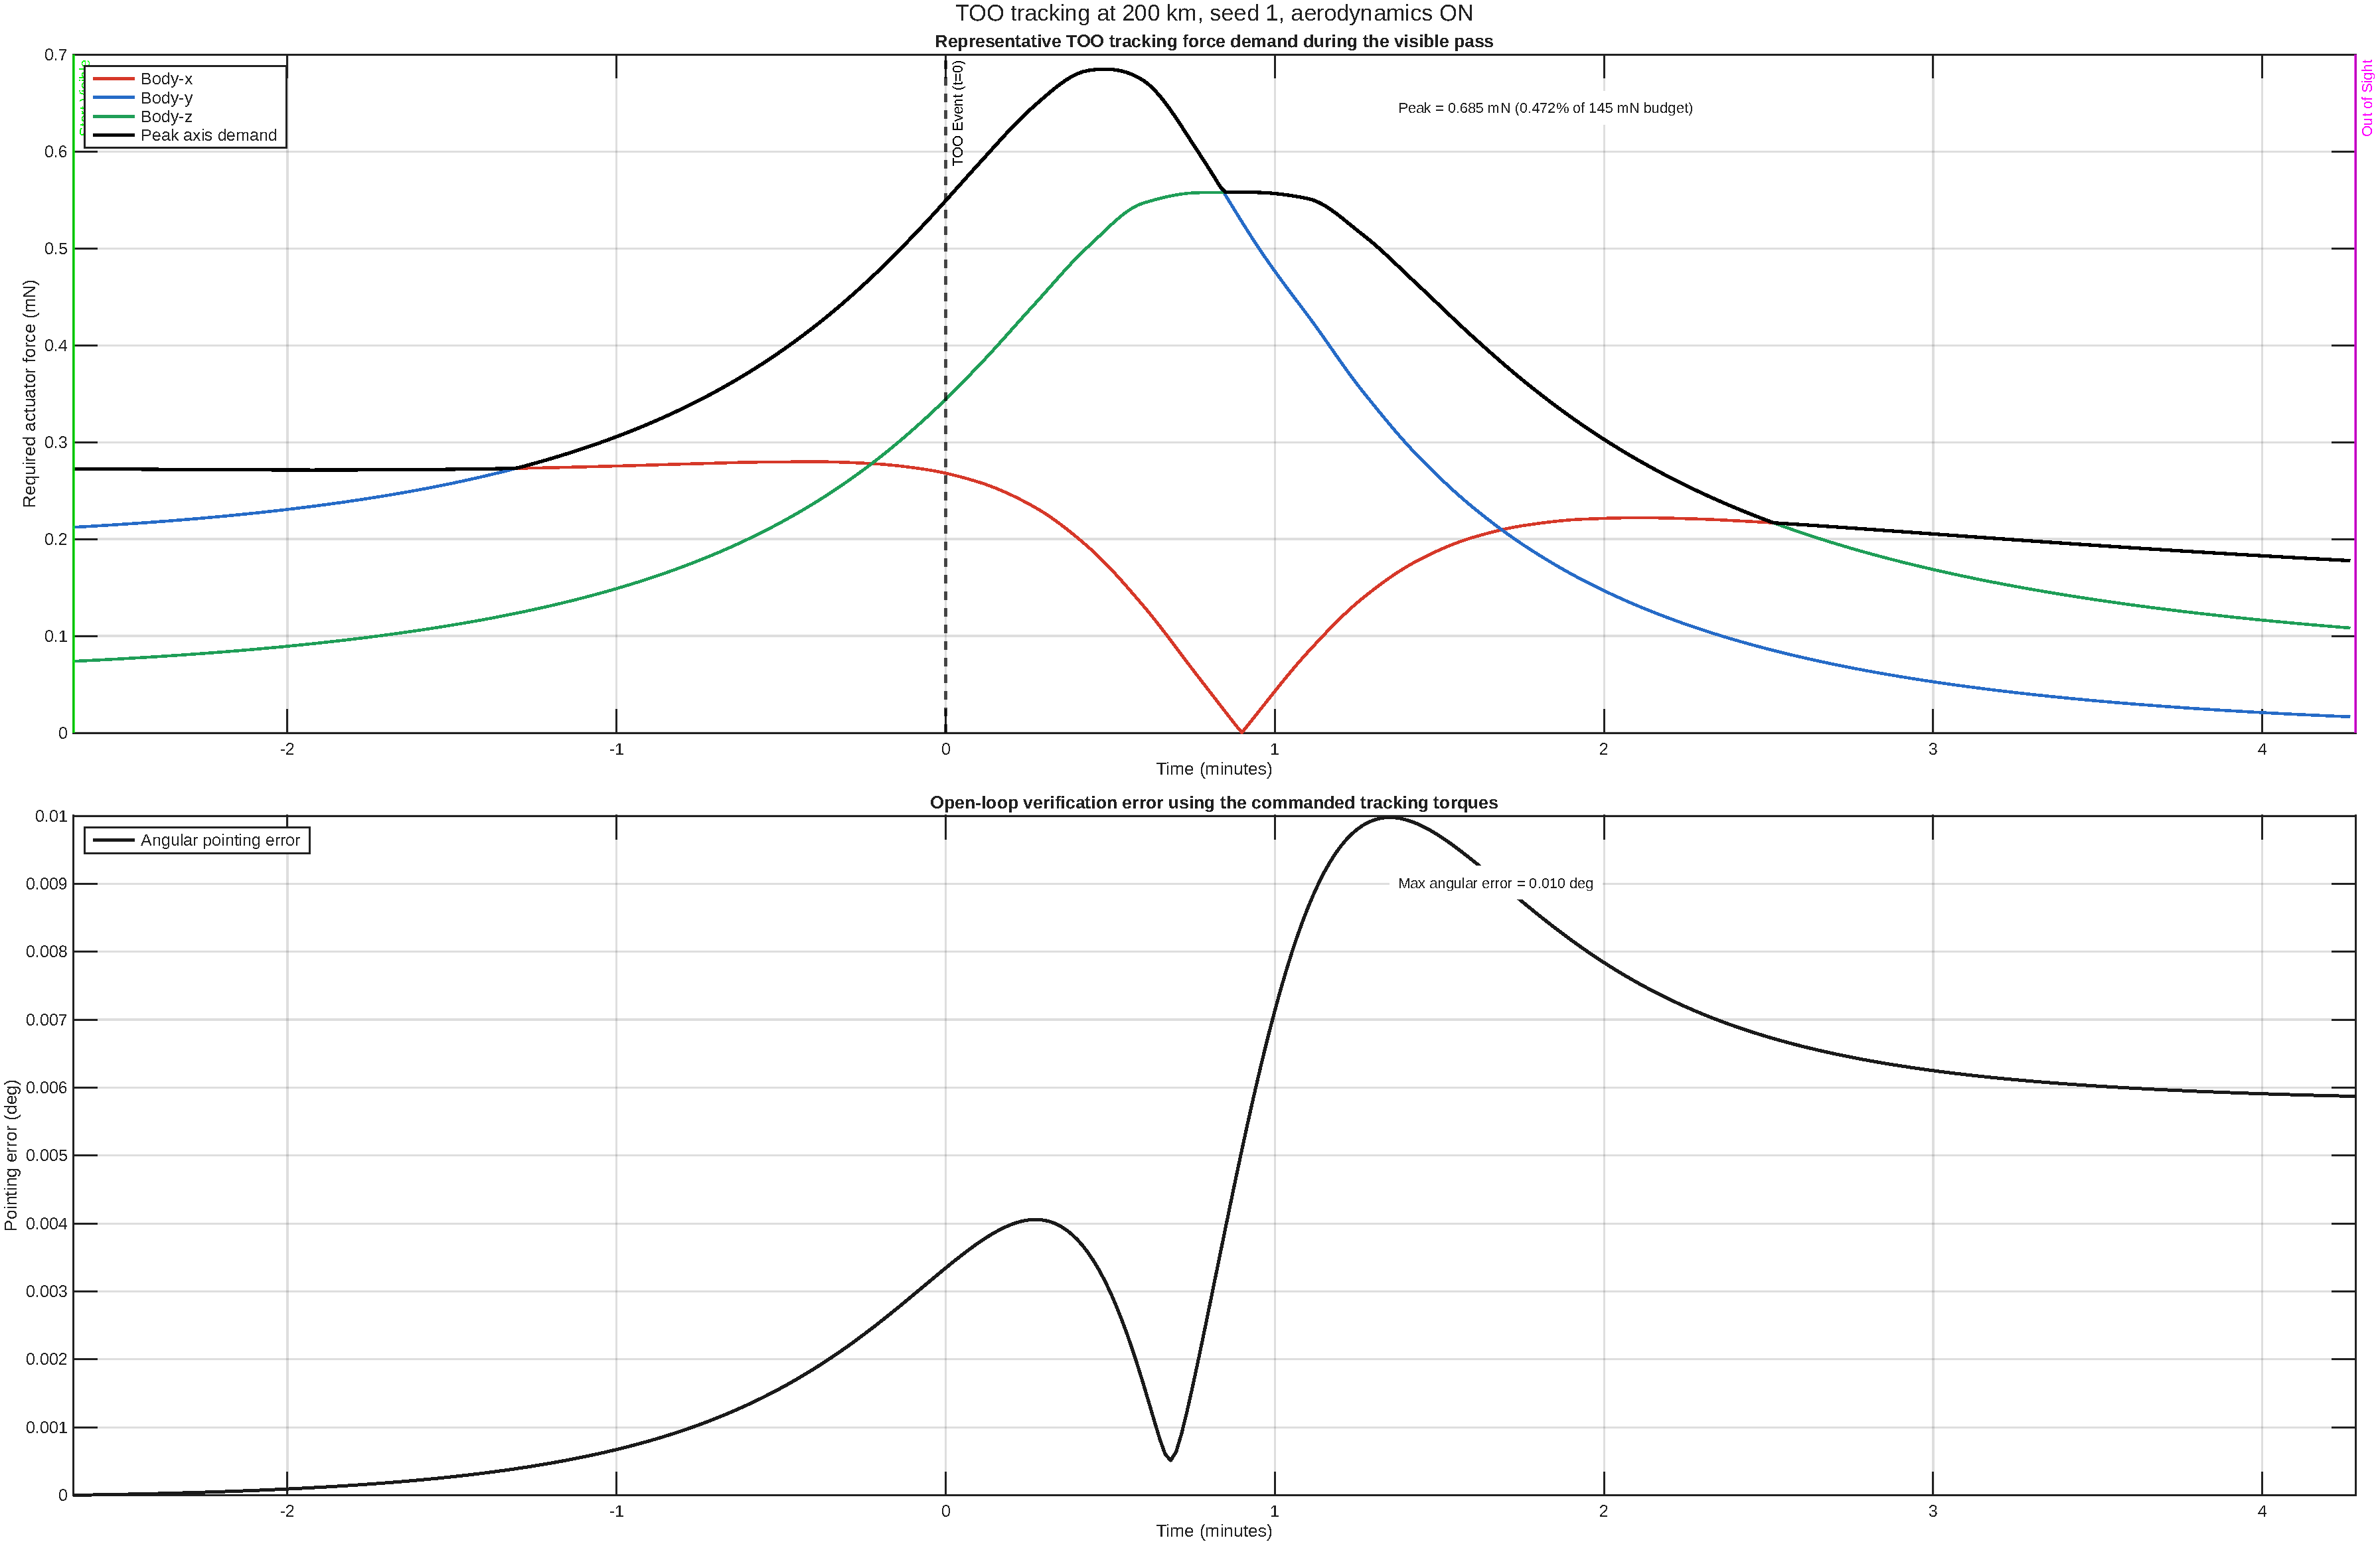
\includegraphics[width=0.75\textwidth]{too_tracking_force_and_error_seed_1_aero_on}
\caption{Seeded \SI{200}{\kilo\meter} TOO continuous-tracking case. The peak actuator force remains below \SI{1}{\milli\newton}, and the open-loop verification accuracy is approximately \SI{0.010}{\degree}.}
\label{fig:tracking-case}
\end{figure*}

The more operationally demanding case is the slew-to-track handoff. A nominal match time is selected from the visibility geometry using a three-quarter visibility rule, and nearby feasible solutions are scanned to confirm the local behavior of the minimax objective. Figure~\ref{fig:handoff-scan} shows the seeded \SI{200}{\kilo\meter} case with aerodynamic compensation included in the scan metric. The selected match occurs at \SI{193}{\second} (\SI{3.22}{\minute}) after event onset. The scan reveals that the full peak actuator-force equivalent is approximately \SI{0.615}{\milli\newton}, while the maneuver-only component contributes approximately \SI{0.071}{\milli\newton}; aerodynamic compensation therefore dominates the total force requirement.

\begin{figure*}[!htb]
\centering
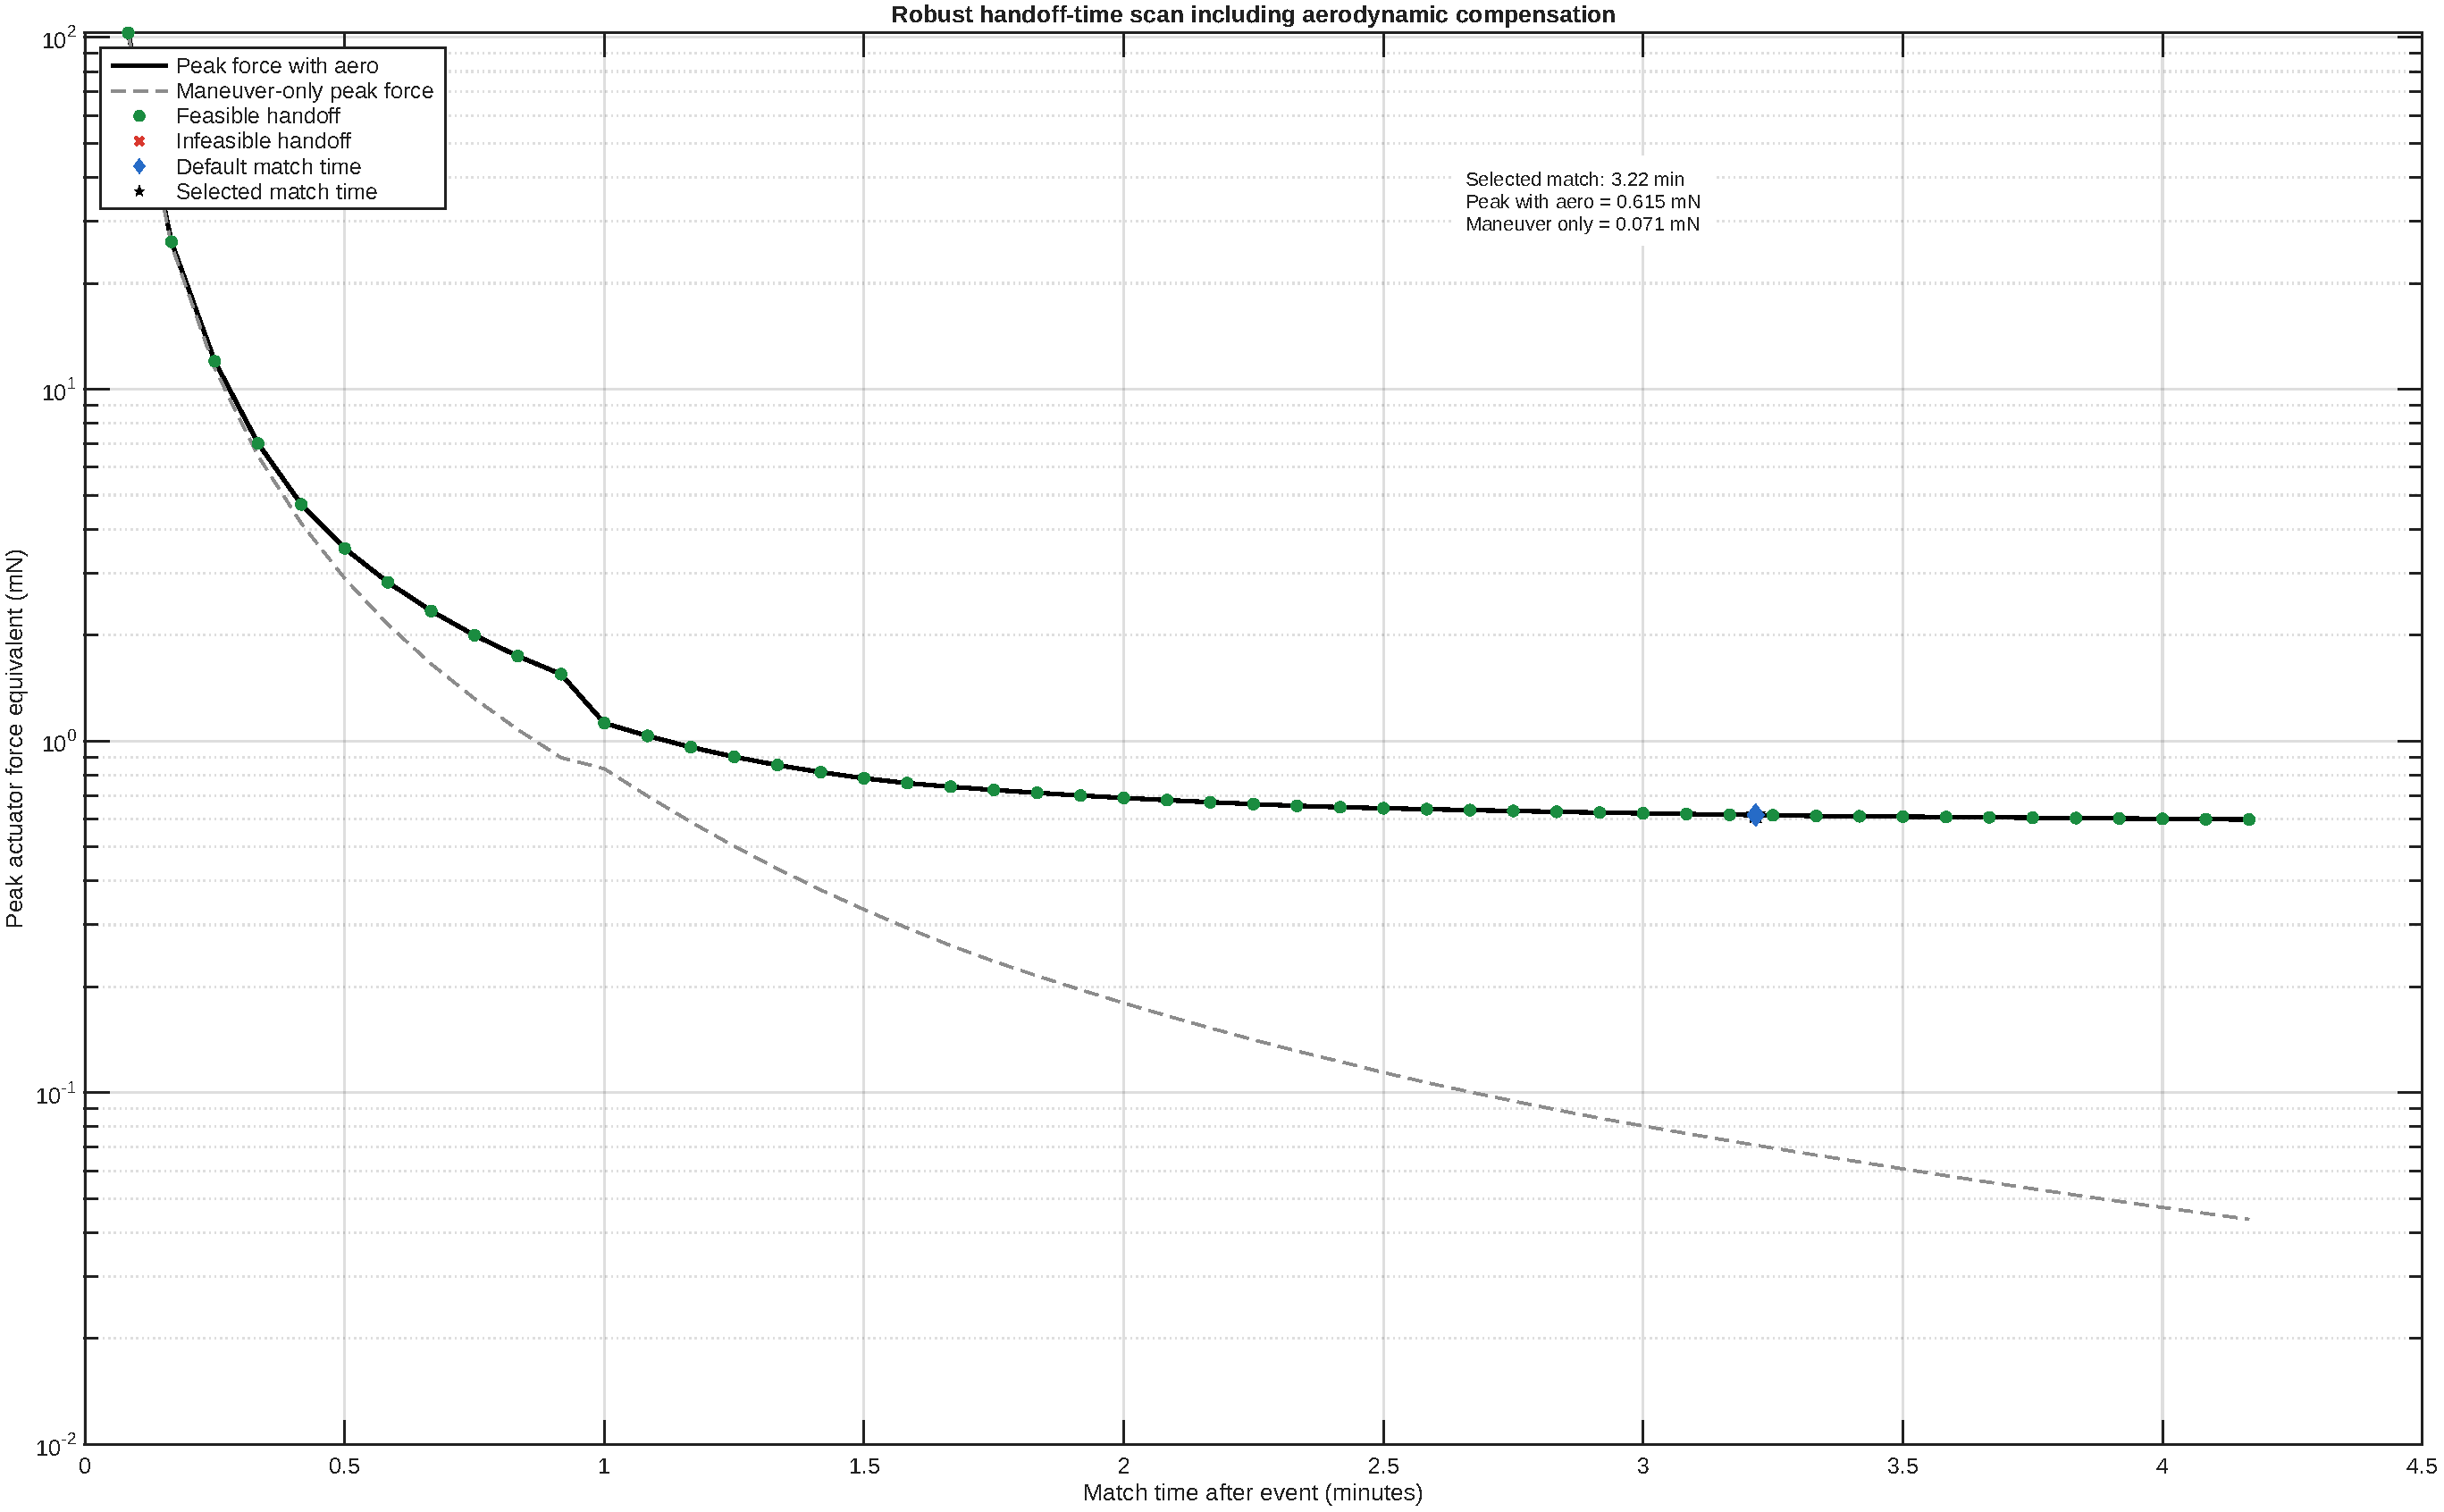
\includegraphics[width=0.75\textwidth]{too_minimax_handoff_scan_seed_1_aero_on}
\caption{Seeded \SI{200}{\kilo\meter} match-time scan for the TOO slew-to-track transition. The solid curve includes aerodynamic compensation; the dashed curve shows the maneuver-only component. The default and selected match times coincide for this seed.}
\label{fig:handoff-scan}
\end{figure*}

Figure~\ref{fig:slew-torque-case} shows the corresponding torque history. The match attitude error is approximately $4.91 \times 10^{-5}$~deg, the post-match maximum pointing error is \SI{0.0183}{\degree}, and the full-case peak actuator force is \SI{0.617}{\milli\newton}, only 0.43\% of the \SI{145}{\milli\newton} budget.

\begin{figure*}[!htb]
\centering
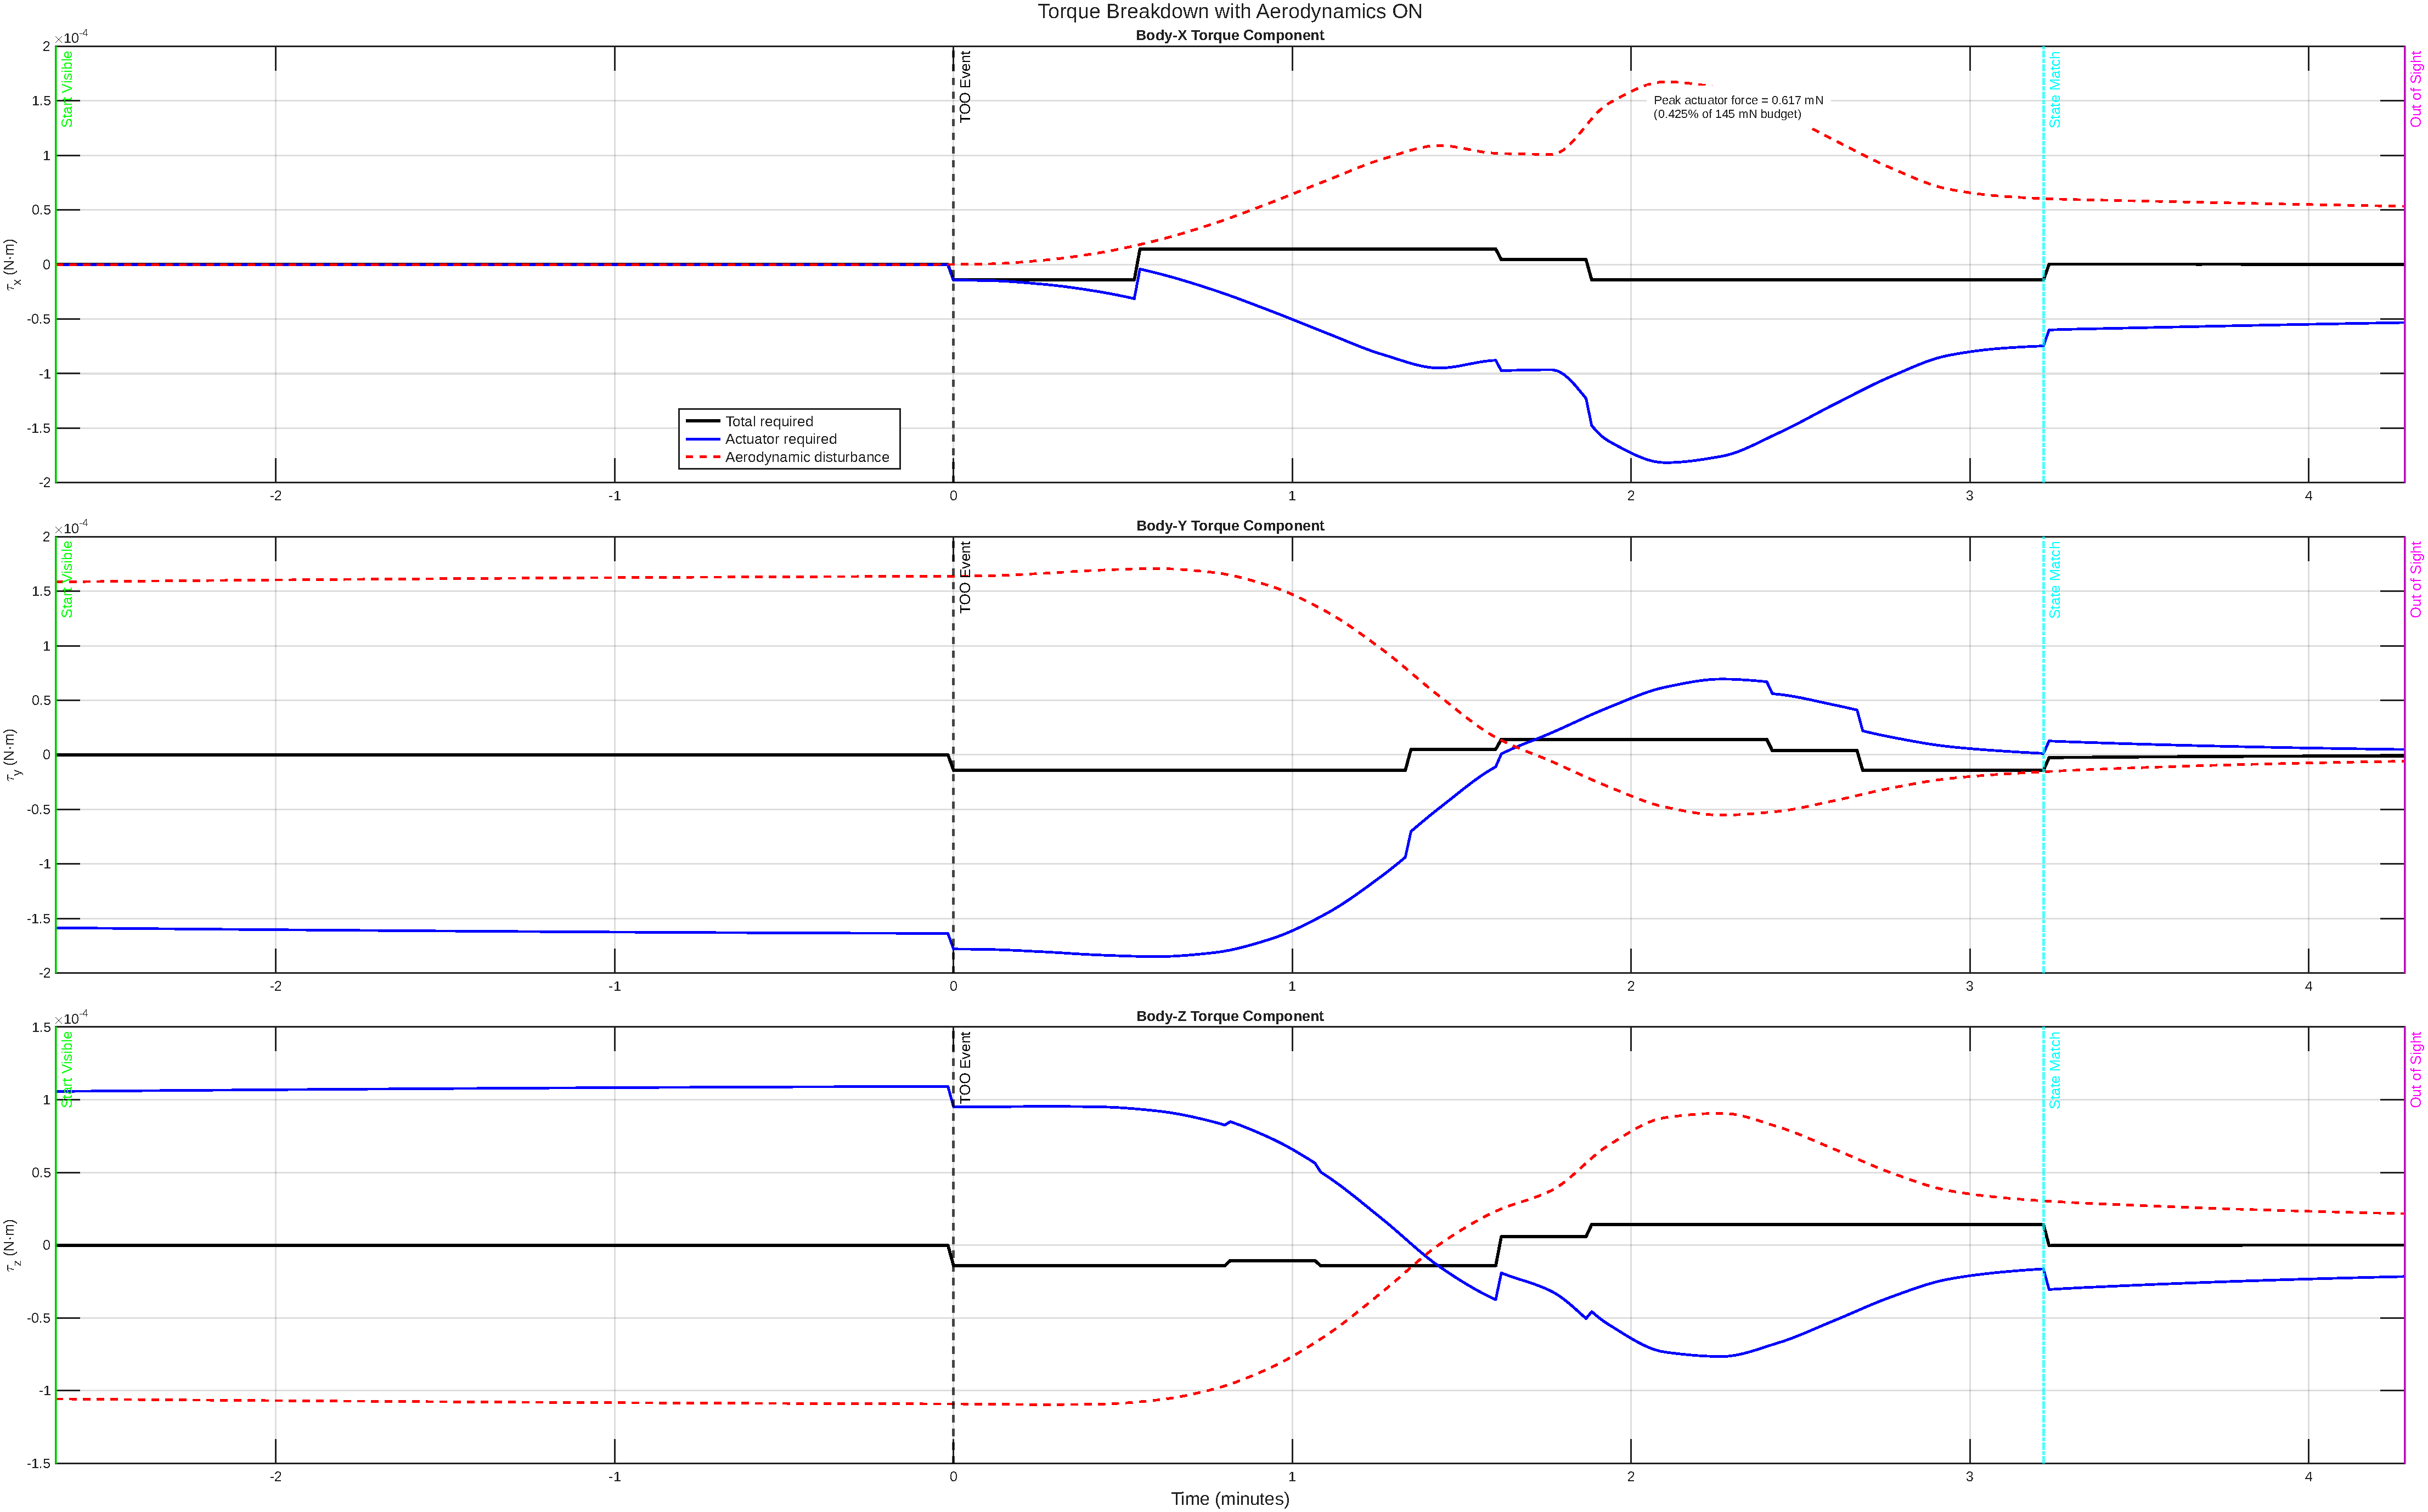
\includegraphics[width=0.75\textwidth]{too_minimax_torque_breakdown_seed_1_aero_on}
\caption{Seeded \SI{200}{\kilo\meter} slew-to-track torque history. Aerodynamic compensation dominates the torque budget; the full case remains below a \SI{0.617}{\milli\newton} peak actuator-force equivalent.}
\label{fig:slew-torque-case}
\end{figure*}

Collectively, the tracking and slew-to-track results reinforce the same conclusion as the analytic and altitude sweeps: instantaneous force authority is not the dominant constraint for the modeled \SI{200}{\kilo\meter} VLEO mission.

%--------------------------------------------------------------------------------------
\subsection{Endurance limits under continuous aerodynamic compensation}

The endurance analysis yields a qualitatively different picture. Figure~\ref{fig:lifetime} shows that the orbit-averaged total thrust required to offset aerodynamic forces and torques decreases strongly with altitude, but the resulting mission life remains short for low- to moderate-$I_{sp}$ ion thrusters.

At \SI{170}{\kilo\meter}, the average total thrust requirement is \SI{19.188}{\milli\newton}, yielding a propellant-limited life of only 6.74~days for the $I_{sp}=\SI{760}{\second}$ case and 26.62~days for the $I_{sp}=\SI{3000}{\second}$ case. At \SI{200}{\kilo\meter}, the average total thrust decreases to \SI{6.919}{\milli\newton}, but life remains only 18.70 and 73.82~days for the same two cases. The advanced $I_{sp}=\SI{19300}{\second}$ case is substantially more favorable (171.24~days at \SI{170}{\kilo\meter} and 474.89~days at \SI{200}{\kilo\meter}), but this performance level corresponds to an advanced high-power concept rather than a near-term CubeSat-class baseline \cite{ds4goverview}.

\begin{figure*}[!htb]
\centering
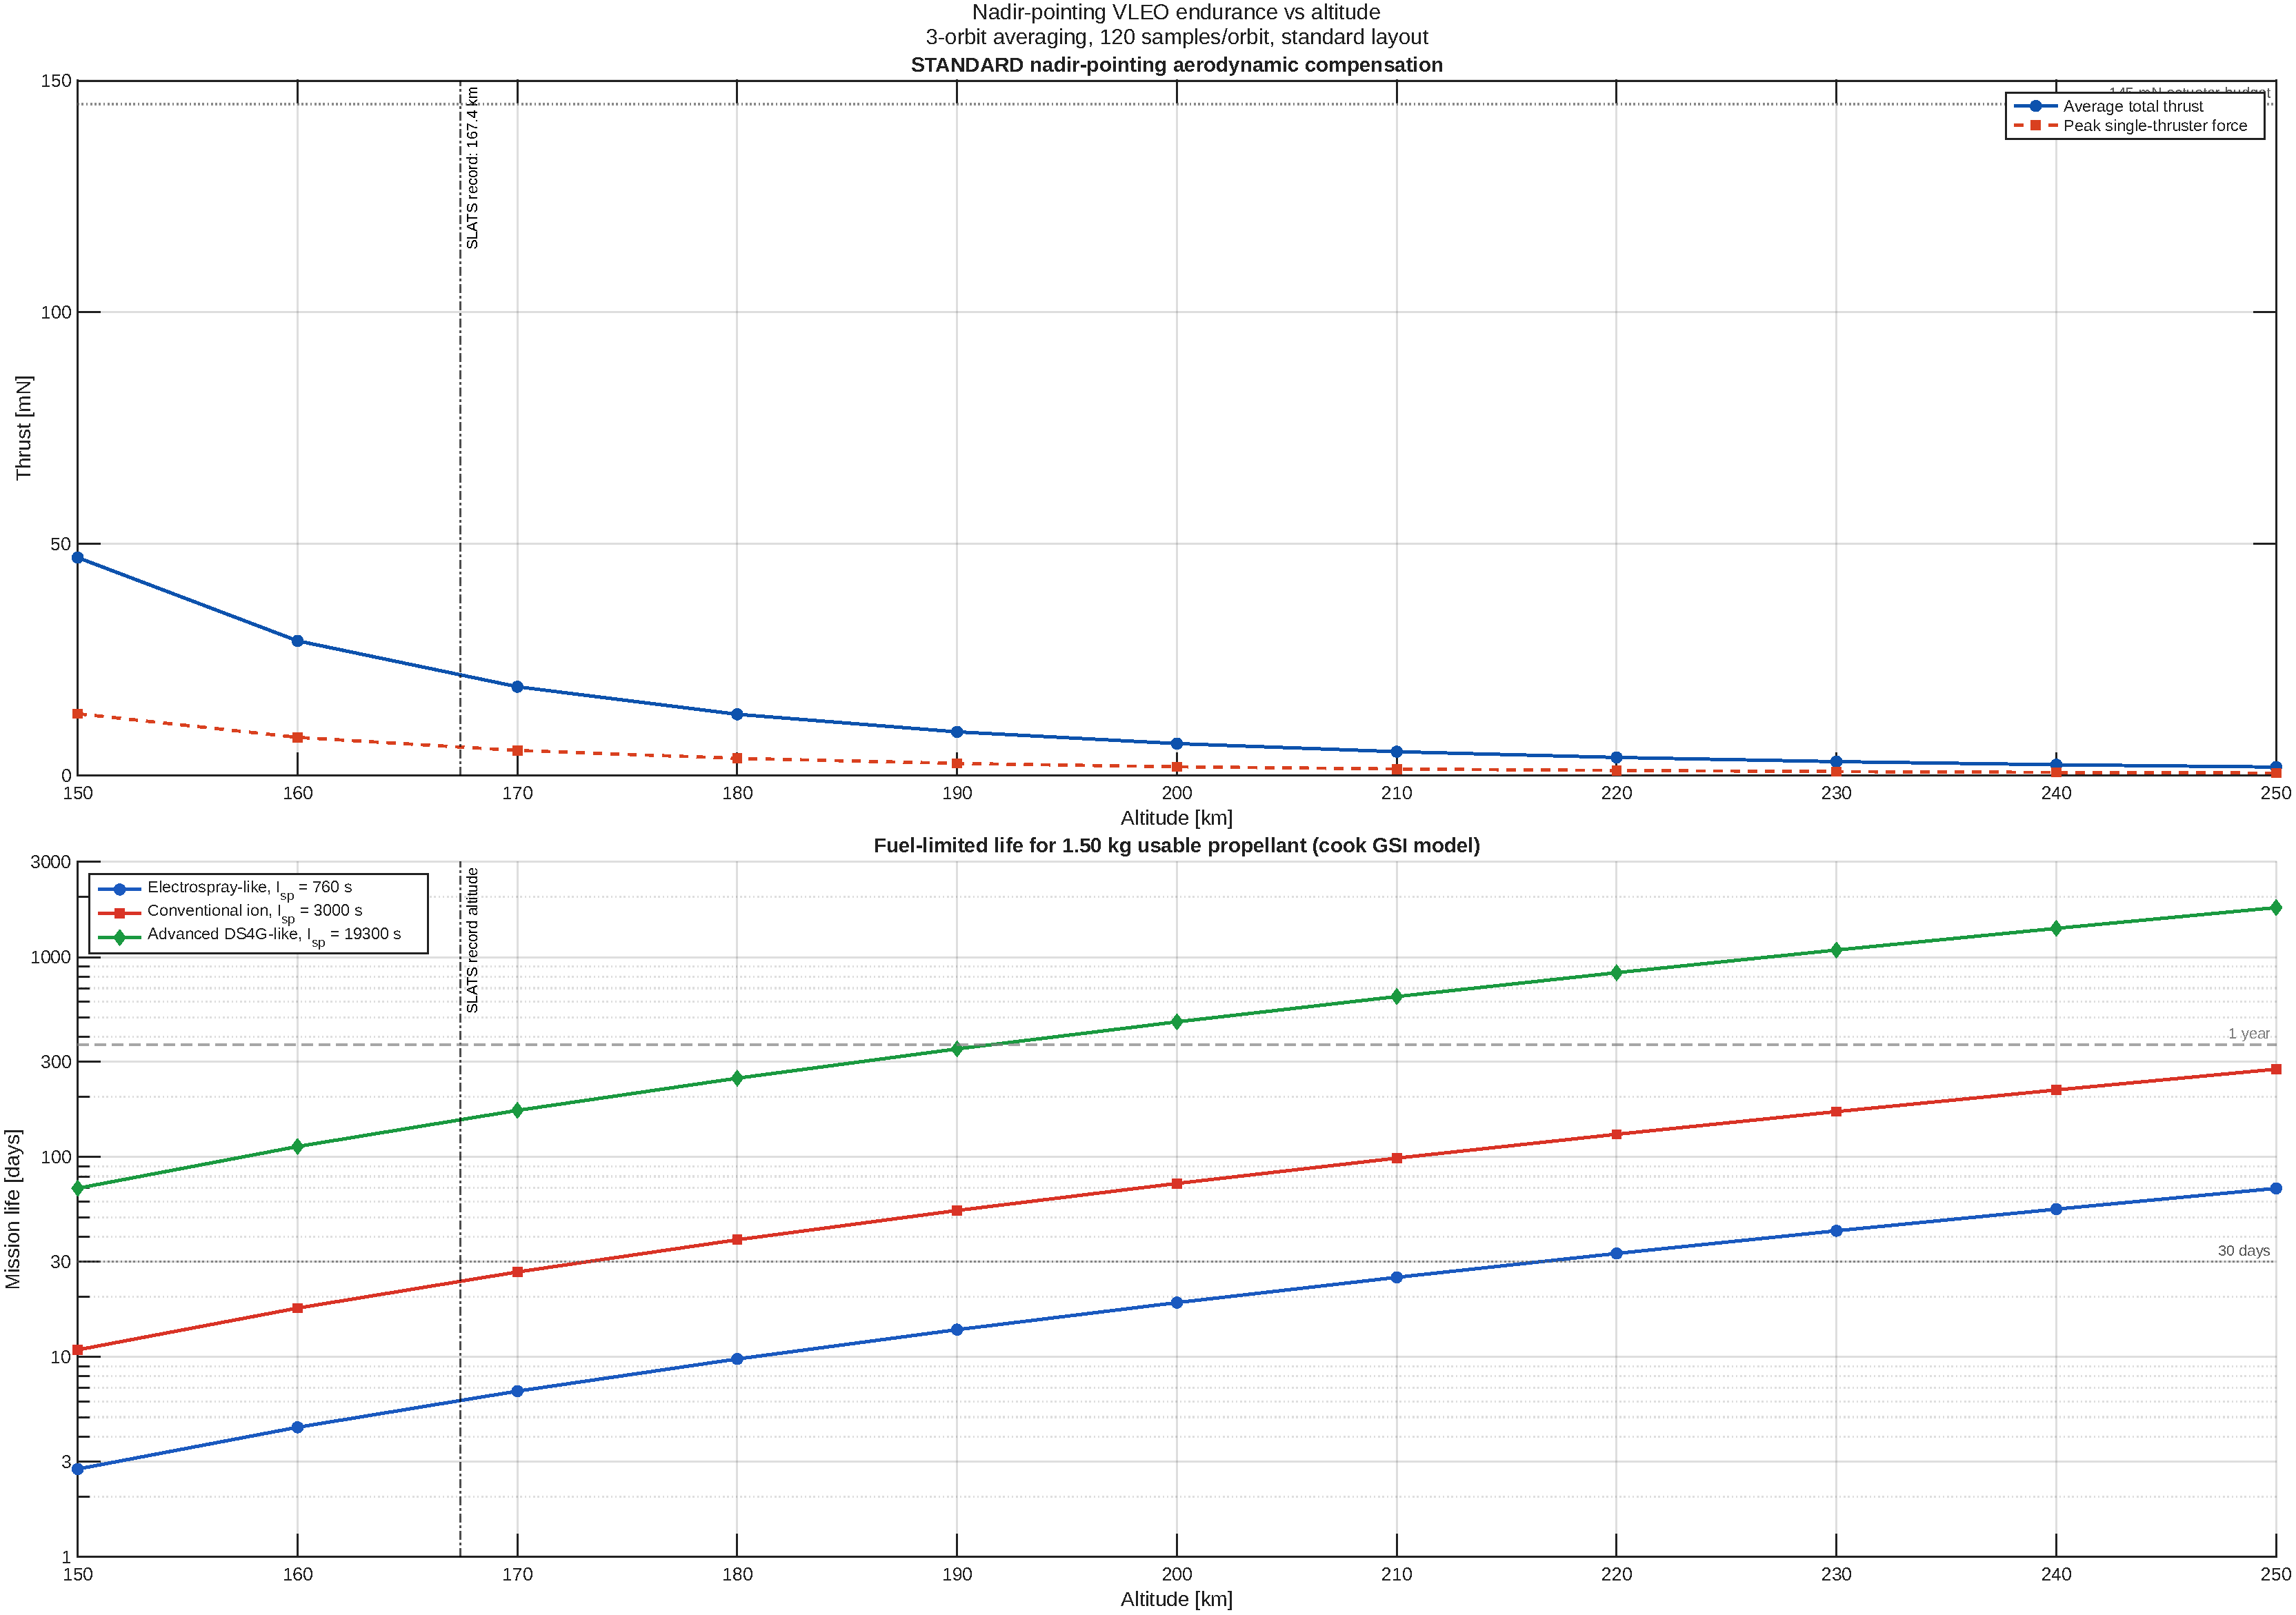
\includegraphics[width=0.75\textwidth]{nadir_pointing_lifetime_vs_altitude}
\caption{Nadir-pointing VLEO endurance versus altitude for three specific-impulse cases. The force demand is modest above the deepest VLEO regime, but sustained aerodynamic compensation drives short mission life for the $I_{sp}=\SI{760}{\second}$ and $I_{sp}=\SI{3000}{\second}$ cases.}
\label{fig:lifetime}
\end{figure*}

This endurance result is the central finding of the study. It demonstrates that VLEO maneuvering and tracking can be feasible from a force standpoint while remaining operationally constrained by propellant-limited mission duration.

%======================================================================================
\section{Discussion} \label{sec:discussion}

The results delineate two distinct regimes for the VLEO ion-thruster problem.

In the peak-force regime, the findings are encouraging. For the modeled 6U vehicle, the \SI{145}{\milli\newton} budget provides ample margin for representative \SI{200}{\kilo\meter} tracking and event-driven slew-to-track operations, and it remains adequate for nadir-pass TOO tracking down to approximately \SI{112.7}{\kilo\meter}. The modeled maneuver force requirements are therefore compatible with high-end ion-thruster-class actuation.

In the endurance regime, the findings are unfavorable. The VLEO aerodynamic environment imposes continuous propellant consumption, and the resulting mission lives are short for the $I_{sp}=\SI{760}{\second}$ and $I_{sp}=\SI{3000}{\second}$ cases. The governing design question is therefore not whether the ion thruster can execute a given maneuver, but how long the mission can remain in the useful VLEO altitude band while performing those maneuvers. For the configuration studied here, the answer is typically measured in days to weeks rather than in operationally meaningful durations.

These findings carry several system-level implications:
\begin{enumerate}
    \item Ion thrusters are plausible as a source of VLEO attitude-control authority, particularly for large-angle slews and aerodynamic disturbance rejection.
    \item Ion thrusters alone are a poor match for sustained low-altitude missions unless the spacecraft carries a substantially larger propellant fraction, operates at higher altitude, or employs propulsion with dramatically higher $I_{sp}$ than conventional CubeSat-class ion systems.
    \item Hybrid architectures remain the more attractive system-level solution. Reaction wheels or other momentum-storage devices can absorb fast attitude transients, while electric propulsion is reserved for drag compensation and slower momentum management.
\end{enumerate}

The study also has limitations that should be acknowledged. It does not size power-processing units, solar arrays, or thermal-rejection hardware; it does not model throttling bandwidth, plume impingement, minimum impulse bit, or duty-cycle constraints; and it uses a single deterministic seeded tracking geometry for the illustrative figures. These omissions do not invalidate the central conclusions, but they are relevant if the analysis is extended from force-feasibility assessment to flight-system design. In practice, these additional constraints are likely to make ion-thruster-only architectures less attractive rather than more so.

%======================================================================================
\section{Conclusion} \label{sec:conclusion}

This paper evaluated ion-thruster-only maneuvering for a \SI{12}{\kilogram} 6U CubeSat in VLEO using analytic slew limits, target-tracking simulations, and propellant-limited endurance estimates. The instantaneous maneuver results are favorable: worst-axis \SI{180}{\degree} slews complete in \SI{6.13}{\second}, the illustrative \SI{200}{\kilo\meter} tracking case requires only \SI{0.685}{\milli\newton}, and the slew-to-track handoff requires \SI{0.617}{\milli\newton} peak actuator force with an aerodynamic-aware scan selecting a \SI{193}{\second} match time. In that force-feasibility sense, VLEO maneuvering is achievable with ion-thruster-class actuation.

The mission-life result constitutes the dominant constraint. Continuous aerodynamic compensation in VLEO drives short endurance for the $I_{sp}=\SI{760}{\second}$ and $I_{sp}=\SI{3000}{\second}$ cases, even though the corresponding peak maneuver forces remain well within budget. Ion thrusters can therefore render VLEO maneuvers feasible, but ion thrusters alone do not make sustained VLEO missions attractive for the modeled CubeSat configuration. For practical VLEO missions, the more credible engineering path is a hybrid control architecture, operation at higher altitude, a larger propellant allocation, or an electric-propulsion system with substantially higher effective performance than current small-satellite ion thrusters.

%======================================================================================
\section*{Acknowledgments}

% TODO: Add acknowledgments here.

\bibliography{vleo_ion_thruster_refs}

\end{document}
